%%Packages
\documentclass[11pt, a4paper]{article}

% Papierformat und Seitenränder
\usepackage[verbose,a4paper,top=25mm,bottom=25mm,left=30mm,right=30mm]{geometry}
\usepackage[utf8]{inputenc}
\usepackage[T1]{fontenc}

%Legt die Schriftart auf ``Latin Modern'' fest
\usepackage{lmodern}

%1,5 facher Zeilenabstand
%\usepackage[onehalfspacing]{setspace}
% Einfacher Zeilenabstand
\usepackage[singlespacing]{setspace}

%Für neue Rechtschreibung und deutsche Silbentrennung
\usepackage[ngerman]{babel}

%Ermöglicht das Einbinden von Grafiken
\usepackage{graphicx}
% Um Grafiken fließender Text
%\usepackage{wrapfig}

% Erhöht maximale Lückengröße zwischen Wörtern
%\setlength\emergencystretch{1em} 

% Für Zitate
\usepackage[round]{natbib}
\bibliographystyle{Bibliographystyle}
%\setlength{\bibinitsep}{\baselineskip}

% %Für Anhänge
% %\usepackage[titletoc,title]{appendix}

% %Nummeriert alle Ebenen von Part (-1) bis Subparagraph (5)
% \setcounter{secnumdepth}{3}
% %Nimmt alle Ebenen von Part (-1) bis Subparagraph (5) ins Inhaltsverzeichnis auf
% \setcounter{tocdepth}{3}

% %Inkludiert das Literaturverzeichnis ins Inhaltsverzeichnis
% %\usepackage[nottoc]{tocbibind}
% %Referenz: ftp://ftp.tex.ac.uk/tex-archive/macros/latex/contrib/tocbibind/tocbibind.pdf

% % Für sehr, sehr viel besseren Blocksatz
% \usepackage[activate={true,nocompatibility},final,tracking=true,kerning=true,spacing=true,factor=1100,stretch=10,shrink=10]{microtype}
% % activate={true,nocompatibility} - activate protrusion and expansion
% % final - enable microtype; use "draft" to disable
% % tracking=true, kerning=true, spacing=true - activate these techniques
% % factor=1100 - add 10% to the protrusion amount (default is 1000)
% % stretch=10, shrink=10 - reduce stretchability/shrinkability (default is 20/20)

% % Macht Leerzeilen zu 'richtigen' Absätzen
% \usepackage{parskip}

% %Einzug der Fußnoten
% %\usepackage[hang, bottom]{footmisc}
% %\setlength{\footnotemargin}{15pt}

% %Fußnoten von Grafiken auf derselben Seite
% \usepackage{afterpage}

% % URL-Paket
% \usepackage[colorlinks,        % Links ohne Umrandungen in zu wählender Farbe
% 	linkcolor=black,   % Farbe interner Verweise
% 	filecolor=black,   % Farbe externer Verweise
% 	citecolor=black,
% 	urlcolor=black]{hyperref} 
	
% %Erstellung eines Glossars
% %\usepackage[nomain, acronym, nonumberlist, toc, section=section, nopostdot]{glossaries}
% %\renewcommand*{\glsgroupskip}{}% no extra line skip between clusters
% %\makeglossaries


% %\input{Glossar.tex}
% %\input{Abkürzungen.tex}

% %Bessere Beschreibungslisten
% %\usepackage{enumitem}

% %Erstellung von Tabellen
% \usepackage[margin=00pt,font=small,labelfont=bf, position=below, skip=3pt, justification=justified]{caption}
% \usepackage{booktabs} % Schickere Linien in Tabellen
% \usepackage{colortbl} % Farben in Tabellen
% \usepackage{tabularx}
% %\usepackage{multirow}

% % Kapitelweise Nummerierung von Abbildungen
% %\usepackage{chngcntr}
% %\counterwithin{figure}{section}

% %Einbinden von externen PDF-Dateien
% \usepackage{pdfpages}

% % Überschriftenformatierung ermöglichen
% %\usepackage{titlesec}

% %Subparagraphen kursiv
% \titleformat*{\subparagraph}{\itshape}

% %Blindtext
% \usepackage{blindtext}

% %Mathematische Symbole
% \usepackage[geometry]{ifsym}

% %Farbiger Text
% \usepackage{color}
% \definecolor{grau}{gray}{.6}

% %Fußnoten ohne Ziffer
% \makeatletter
% \def\blfootnote{\gdef\@thefnmark{}\@footnotetext}
% \makeatother

% % EINSTELLUNGEN
% % -------------------------------------------

% % Verhindert Hurenkinder und Schusterjungen recht zuverlässig
% \widowpenalty = 10000
% \clubpenalty = 10000
% \interfootnotelinepenalty = 10000

% %Einzug in Beschreibungslisten global festlegen
% \setlist[description]{leftmargin=\einzug}

% %Abstand zwischen Gleitobjekten und Text
% \setlength{\intextsep}{20pt}

\documentclass[11pt, a4paper]{article}

\usepackage[utf8]{inputenc}
\usepackage[T1]{fontenc}
\usepackage{lmodern}
\usepackage[singlespacing]{setspace}
\usepackage{parskip}
\usepackage{graphicx}
\usepackage{amsmath}
\usepackage{float}
\usepackage{makecell}
\usepackage[activate={true,nocompatibility},final,tracking=true,kerning=true,spacing=true,factor=1100,stretch=10,shrink=10]{microtype}

\widowpenalty = 10000
\clubpenalty = 10000
\interfootnotelinepenalty = 10000

\pagenumbering{Roman}

\title{Developing a Deep Learning Process for the Segmentation of 3D MR images}
\author{Paul-Louis Pröve}

\begin{document}

    \begin{titlepage}
    \centering
    
\includegraphics[width=0.4\textwidth]{imgs/fhw.png}\par
    \vspace{1cm}
    {\scshape\Large Bachelor Thesis\par}
    \vspace{2cm}
    {\bfseries\Huge Automated Segmentation of Bone Matter in 3D MR Images using Convolutional Neural Networks\par}
    \vspace{2cm}
    {\itshape\Large Paul-Louis Pröve\par}
    mail@plpp.de\par
    \vfill
    supervised by\par
    Prof. Dr. Dennis Säring\par
    dsg@fh-wedel.de\par
    \vspace{1cm}
    Hamburg,\par \today\par
    \end{titlepage}

\section{Abstract}

Password attacks are at the edge of accessing someones secrets. By learning to judge the strength of a password and by understanding how hackers execute attacks, users can make better estimations on how safe they are.

The entropy is widely used to measure how safe a password is, but many sources draw inaccurate conclusions between the entropy of a random password and the strength of a password that was chosen by a person. It is important to understand how these two differ and why realistic password strength is often hard to determine.

Todays hardware gives hackers incredibly powerful machines to launch different types of password attacks. Common password patterns lower possible permutations by such a magnitude that even seemingly safe passwords can be successfully attacked. In combination with frequently used passwords and personal information, hackers can further increase the effectiveness of their attacks.

By explaining common terminologies and analysing different datasets we will look at password attacks from the perspective of users, system administrators and hackers. All three benefit by understanding how the others operate in practice.

\newpage

\tableofcontents
\newpage

%\listoffigures
%\newpage

\pagenumbering{arabic}

\section{Introduction}

Recent advances in Artificial Intelligence have led to fully automated workflows that often exceed human performance. State of the art neural networks can classify images into thousands of categories more accurate and magnitudes faster than we can. They translate text between hundreds of languages, navigate cars autonomously through cities and detect intruders in computer systems. In most of these cases they have been trained on tens of thousands or even millions of data samples to reach their accuracy. 

Neural networks have also found great success in the medical field, where the requirements are quite different and the data sets are often much smaller. Although the same techniques can be applied, they need to be adjusted to match a particular problem. In many applications neural networks have been setting the current state of the art when it comes to different segmentation or classification tasks.

The age assessment is a challenging procedure to determine the chronological age of a person lacking legal documents. It exists to afford children provisions they are entitled to by law and to prevent adults from taking unwarranted advantage of these benefits. There is no method that offers an exact identification of the age, but several assessments are currently used that can be separated in two groups.

Personal interviews or examinations are held to gain an observation of physical or psychological features of the person. Besides the fact that these practices include a high amount of manual work comes the problem that they are also subjective to the person conducting the test. The other type of assessments use X-rays to observe physical traits like the collar bone, teeth or carpal growth plates. Besides that these images are also analyzed manually comes the problem that X-rays are considered an invasive imaging method because they require the exposure of ionizing radiation. In some european countries like Germany, these recordings can only be induced in a criminal matter and therefore not be used for refugee applications.

As such, there is a high demand for a fully automated, unprejudiced and non-invasive method for accurately determining the age of a person.

Based on this idea, I was introduced to a data set of MRIs showing the right knee of several candidates. In contrast to CT or X-ray, MRI is considered non-invasive. Similar to the carpal analysis, the three bones around the knee show growth plates which have been used as indicators for the age of a person. One downside of MRIs in this context is that they are much more sensitive to non-bone tissue in the human body. 

-----------

The accurate age assessment based on biometric features is a key element in many medical and political

Introduce Field and Context
Summarize previous Research
Define a Research Problem
Introduce the present Research

Statement of the problem: briefly describe problem
Significance of the Study
Objectives of the Study
Time and Place
Scope and Limitation

github link

What is the subject of the paper?
What is the area of interest and what have other researchers found?
How does the current research relate to previous research?
What is the research objective and what hypothesis or research question is being tested?

establish/define any necessary terms/concepts/events/methods etc.
establish your point of view i.e. your main points (what you are going to argue).
orient your reader to what follows i.e. your main points, how you establish your response, the ideas and arguments to be developed.
have a clear and comprehensive statement of your argument in relation to the set topic.

\newpage

\section{Background*}

This chapter provides an overview of prerequisites and previous work that led to the main task of this thesis. It features a section for the necessary medical knowledge as well as a hierarchical derivation to the appropriate branch in computer science.

\subsection{Medical Knowledge*}

This chapter will briefly explain how the imaging technology works that was used to create the data set and why the growth plates play an elementary role of the long term goal of this study.

\subsubsection{Magnetic Resonance Imaging*}

Magnetic Resonance Imaging (MRI) uses magnetic fields and radio frequencies to probe tissue structure. In contrast to x-ray and CT which require the exposure of ionizing radiation, MRI is a non-invasive imaging method. As such it has become an essential diagnostic imaging modality in the medical field \cite{Westbrook2016}.

96\% of the human body is made up of hydrogen, oxygen, carbon and nitrogen, all of which are referred to as MR active. These elements have an odd atomic mass number giving the nucleus a spin. Due to the laws of electromagnetic induction the motion of unbalanced charge produces a magnetic field around itself. Hydrogen is the element used in MRI, because it is abundant in the human body and its solitary proton in the nucleus gives it a relatively large magnetic moment \cite{Westbrook2016}. 

The positively charged hydrogen particles in water produce a signal when exposed to a strong external magnetic field. This field is supplied by a magnet in the MRI machine aligning the magnetic field of the hydrogen atoms parallel to its own. Gradient coils are used to cause a linear change in the strength of this field. By alternating the current of these coils on three perpendicular axes it is possible to calculate a three-dimensional image of the tissue \cite{Westbrook2016}.

\subsubsection{Growth Plates}

Growth plates are hyaline cartilages at the end of each long bone in the human body. 

\subsection{Computer Science*}

The main task of this thesis revolves around a very specific branch of computer science problems. In this section I want to provide a path to where most of the work will take place. Figure 1 visualizes the hierarchical relationship of the following subsections.

\begin{figure}[H]
\centering
\par

\includegraphics[width=0.8\textwidth]{imgs/cs_hier.png}
\caption{Hierarchical overview where convolutional neural networks and semantic segmentation are placed in the field of computer science}
\par
\end{figure}

\subsubsection{Artificial Intelligence*}

Artificial Intelligence (AI) is understood as the effort of automating a given task that normally needs human intelligence to solve\cite{Chollet2017}. The history of AI goes back to the 1950s, where a certain type called "symbolic AI" started to gain popularity. It was believed that human level intelligence could be achieved through hard-coded rules that programmers specified. 

Taking a complex problem like playing chess and continuing to break it into smaller problems, until they can be solved with known logic. While it was effective for certain tasks, fuzzy problems like image classification, speech recognition or language translation were difficult to tackle. Over the years a new approach was found, which today is referred to as machine learning (ML).

\subsubsection{Machine Learning*}

The concept of classical programming is that an engineer defines a set of rules, called an algorithm, which uses input data to calculate some form of output data\cite{Chollet2017}.

--insert picture--

A machine learning algorithm is an algorithm that is able to learn from data\cite{Goodfellow2016}. It can be used to automatically calculate these rules, so they don't have to be specified by hand. Three components are needed for such an approach.

\begin{itemize}
\item Input data the algorithm is supposed to transform
\item Output data the algorithm is supposed to predict
\item A measurement to validate the performance of a prediction
\end{itemize}

It works by feeding input and output data into a pipeline, which will learn to transform one into the other. With the advantage that no explicit programming is needed to generate the rules, comes the disadvantage that prior input and output data is needed for the initial learning process.

--insert picture--

Machine learning may be applied as an effective method if it's not feasible or possible to define an algorithm by hand and sufficient data is available for training. How much “sufficient” is depends on factors like type of task, complexity of the data, uniformity of the data, type of machine learning algorithm and others.

There are different subparts to machine learning like supervised and unsupervised learning. Supervised learning is used when it's clear what the output data looks like, whereas unsupervised learning can help to find unknown patterns in the data. Examples of supervised learning techniques include linear regression, naive bayes, support vector machines, decision trees, random forests, gradient boosting and artificial neural networks (ANNs). Since the main interest of this study revolves around ANNs, this will be the focus of following chapters.

\subsubsection{Artificial Neural Networks*}

Artificial neural networks are inspired by neurobiological concepts of the human brain. However, they are not models of the human brain. There is no evidence to support that the brain implements anything like the learning mechanisms used in ANNs \cite{Chollet2017}. Artificial neural networks are mathematical frameworks for learning representations from data and one of, if not the only tool in deep learning (DL) --- a subset of machine learning.

The origin of the term deep learning is twofold. On one hand it refers to the fact that ANNs are able to learn "deep" hierarchical information from data. On the other it describes that they show multiple layers of depth within their architecture. ANNs are as old as machine learning itself, but only gained a lot of their popularity in recent years \cite{Chollet2017}.

\begin{figure}[H]
\centering
\par
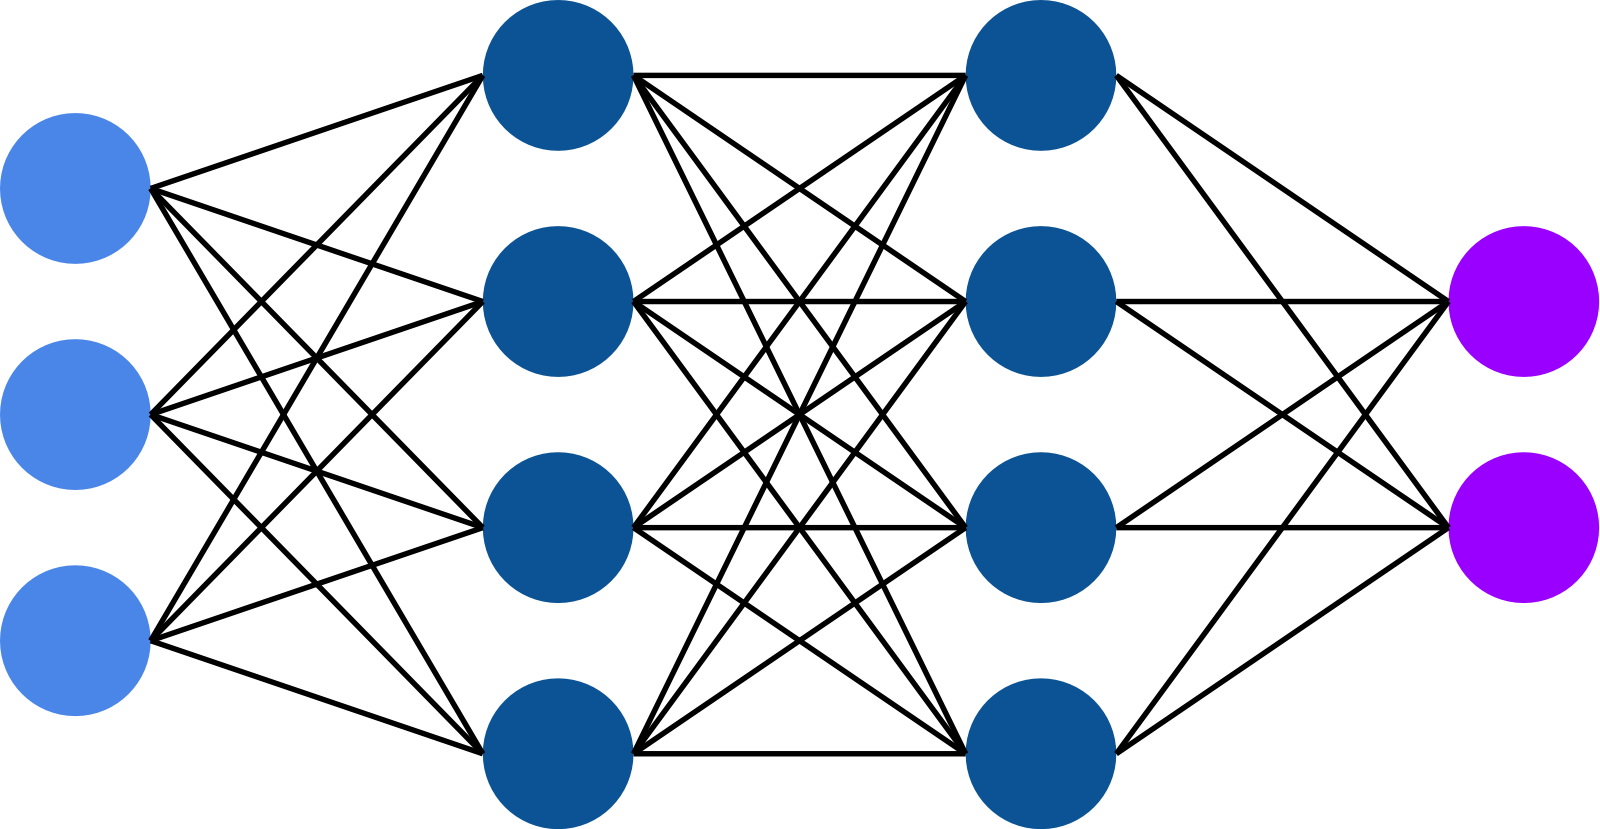
\includegraphics[width=0.8\textwidth]{imgs/ann.png}
\caption{An ANN with 3 input nodes, 2 hidden layers with 4 nodes each and 2 output nodes}
\par
\end{figure}

These dense layers inside artificial neural networks contain entities called nodes that are jointly linked with one another. Every node in a dense layer is connected to each node in the previous and following layer. This structure gives ANNs the capacity to approximate complex mathematical functions and learn global representations in the data. These nodes, also called parameters, can range to hundreds of millions depending on the task.

\subsubsection{Convolutional Neural Networks*}

Convolutional neural networks (CNNs) are a specific type of ANN that use an operation called convolution in at least one of their layers. The first CNN was introduced by Yann LeCunn \cite{LeCun1998} in 1989 at which time it's popularity was limited. In 2012 a CNN called AlexNet \cite{Krizhevsky} won the prestigious ImagetNet competition and these types of networks have been winning ever since.

A convolution is a mathematical operation on two functions of real-valued argument. In deep learning terminology the first function refers to the input and the second function describes the kernel. The output of this operation is called a feature map \cite{Goodfellow2016}.

Convolutions are frequently used in image processing, which is also why they were introduced to visual tasks in the field of deep learning. They allow to learn local patterns in the data instead of treating the input features in a global manner, like dense layers do.

Another type of layer that is frequently used in CNN architectures perform a pooling operation. By doing so the spatial resolution is reduced and only the most relevant features are kept. This is important to keep the size of a CNN manageable.

\subsubsection{Semantic Segmentation*}

CNNs can help to solve different types of supervised machine learning problems of which regression, classification and segmentation are the most common.

A regression describes the prediction of one or multiple continuous outputs. An example for this would be the age prediction of a person based on their knee MRI. Regression is also an important part of object detections, where it's applied to determine coordinates in an image.

A classification sorts the input into one or multiple categories, like predicting if the growth plate is open, partially closed or closed. It can be seen as n parallel regressions where n equals the total number of classes. The continuous output for each class is the probability of the input belonging into this category. For 1 out of n classifications, the most probable category is predicted. For m out of n classifications, a threshold defines at which point a category is predicted.

A segmentation creates an image of identical dimensions as the input and masks specific regions within. Every channel of the output mask belongs to a certain category that is segmented. A segmentation can be seen as a classification of each pixel/voxel. For this study the Femur, Tibia and Fibula needed to be masked from the rest of the MRI content. This is called a semantic segmentation because the process is based on a semantic meaning of objects in the image.

\newpage
\section{Methods}

The purpose of this chapter is twofold. It will discuss the design and processing decisions that were made for the development of this project, while also giving critical insight into how these applied technologies work.

\subsection{Setup}

The workstation included an Intel i5 processor, 16GB of RAM and most importantly a NVIDIA GeForce GTX1060/6GB. Neural Networks can be trained more efficiently on GPUs than CPUs. This is because the simpler but highly parallelized architecture of graphics chips plays in favor for the needed calculations in deep learning \cite{NVIDIA}.

The computer ran Ubuntu 16.04 with the NVIDIA CUDA and cuDNN libraries installed to take advantage of the GPU. As the primary programming language Python 2 was chosen due to its simple syntax and popularity in the deep learning field. The code was briefly tested with Python 3 as well and seemed to work. Keras was used as the framework for training models because its top level syntax allows fast prototyping and testing. The development environment was a Jupyter Notebook, which allowed a flexible execution of code snippets instead of running the entire program for every single change.

The processing of medical image data needed a library that could handle these formats. SimpleITK is a Python binding to the ITK library written in C++. It includes many tools for image processing and is especially popular in the medical field. Other libraries were also used for smaller tasks. A complete listing can be found on the project's GitHub page, where the entire code is available.

\subsection{Data Analysis}

The data set was a collection of three dimensional MR images showing the human right knee. The number of available samples grew during the project. For most of the development time, it included 150 samples that came from 3 different sources. All images were provided in the MHD file format, which is very common in the medical field. It features lossless compression, as well as certain meta information about each image. The resolution of these samples differed from one source to the other.

\begin{table}[h!]
\centering
\begin{tabular}{l l l r r l}
    Source & Prospective & Perspective & Samples & Maps & Resolution \\
    \hline
    Epi    & Yes         & Coronal     & 80      & 40   & 800x800x41 \\
    Jopp   & No          & Coronal     & 65      & 36   & 512x512x24 \\
    Maas   & No          & Sagittal    & 5       & 0    & multiple \\
\end{tabular}
\caption{Details of available images sorted by their source}
\end{table}

The Maas data featured a sagittal perspective, while all other samples were taken coronal. This mattered because the resolution of all images was roughly 20 times lower on the z-axis. The 65 Jopp images were another source of retrospective data, of which 36 had segmentation maps. The origin of this data was a previous study that investigated the condition of the growth plates of Tibia and Femur. A total of 80 MR images were taken specifically for this project. They showed the highest resolution in all dimensions and half of them had segmentation maps.

\begin{figure}[H]
\minipage{0.32\textwidth}
  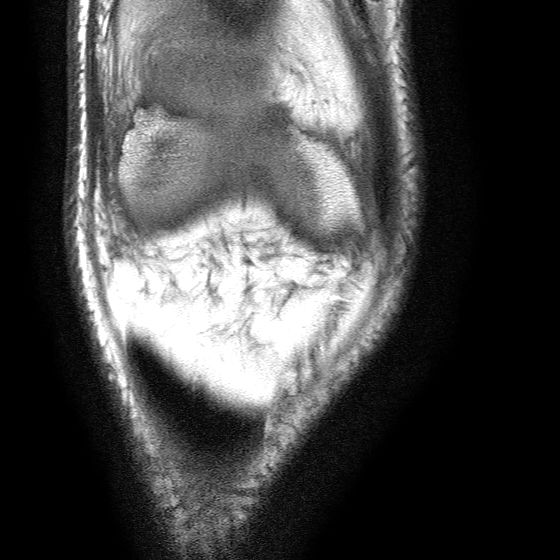
\includegraphics[width=\linewidth]{imgs/3.jpg}
\endminipage\hfill
\minipage{0.32\textwidth}
  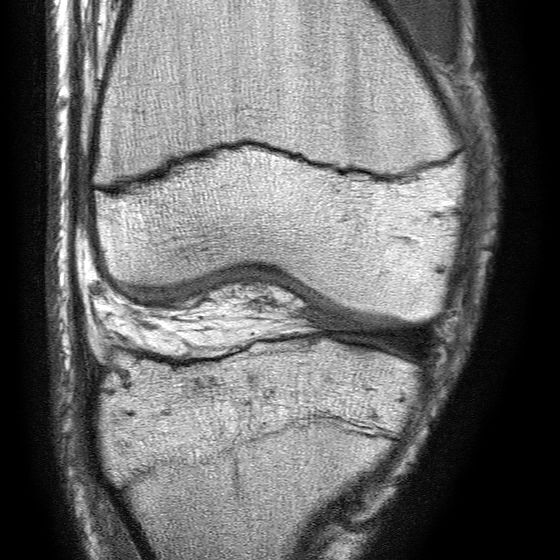
\includegraphics[width=\linewidth]{imgs/10.jpg}
\endminipage\hfill
\minipage{0.32\textwidth}%
  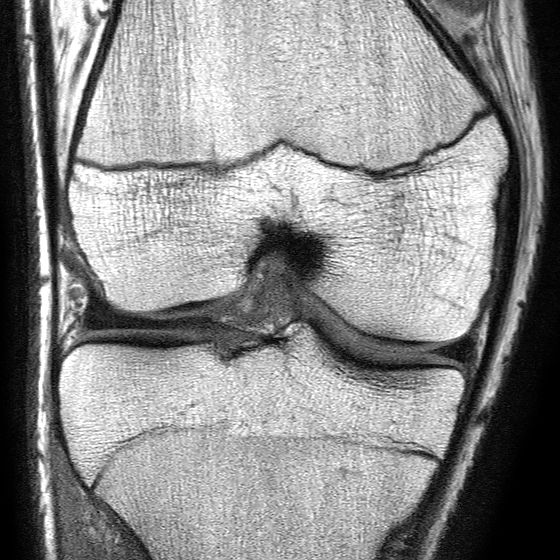
\includegraphics[width=\linewidth]{imgs/17.jpg}
\endminipage
\vspace{0.2cm}
\minipage{0.32\textwidth}
  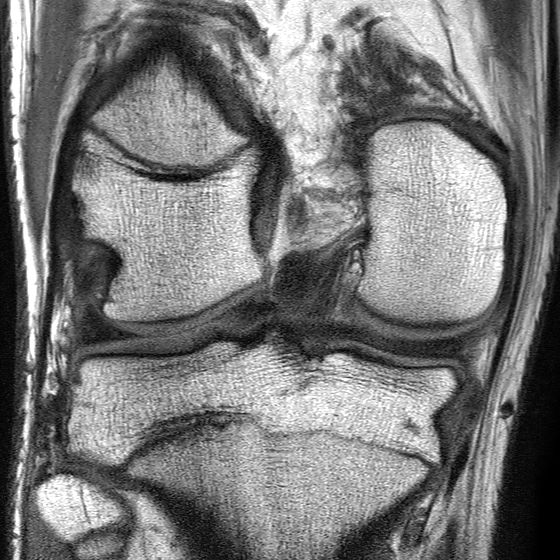
\includegraphics[width=\linewidth]{imgs/24.jpg}
\endminipage\hfill
\minipage{0.32\textwidth}
  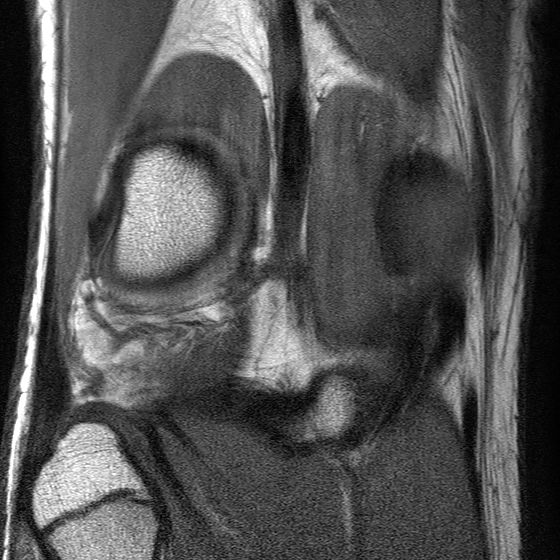
\includegraphics[width=\linewidth]{imgs/31.jpg}
\endminipage\hfill
\minipage{0.32\textwidth}%
  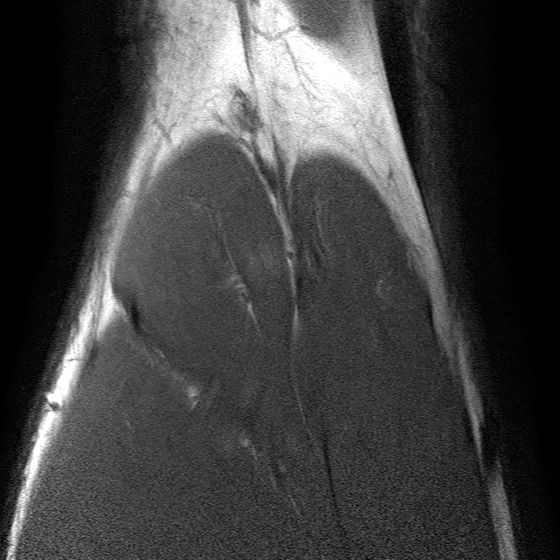
\includegraphics[width=\linewidth]{imgs/38.jpg}
\endminipage
\caption{Six equally distributed slices of a single 3D MRI sample. Femur and Tibia are visible starting at the second image, whereas the Fibula becomes visible in the lower left corner of the 4th image.}
\end{figure}

The total of 76 segmentation maps were all manually labeled by two people. Each mask featured three channels that showed Femur, Tibia, and Fibula separately. They did not segment the entirety of each 3D image but masked a window around the knee cap where the three bones meet.

\begin{figure}[H]
\centering
\par
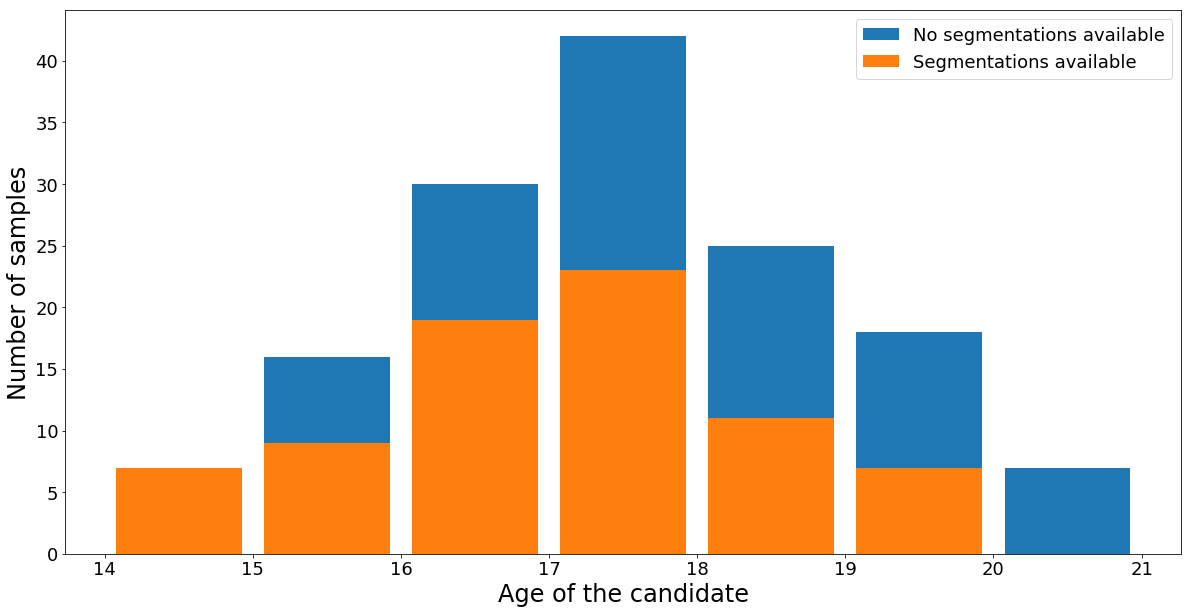
\includegraphics[width=1.0\textwidth]{imgs/age_distr.png}
\caption{Age distribution in the data set. Purple shows the samples for which segmentation maps were available. Blue includes the rest.}
\par
\end{figure}

The candidates chosen for the MRI recordings were all german males between the age of 14 and 20. Their age was normally distributed, and a majority of the candidates were recorded twice roughly a year apart.

\subsection{Preprocessing}

The parameters in a Neural Network commonly range from tens of thousands to hundreds of millions. This complexity allows the model to learn on its own what features of an image are relevant for any given task. It works in conjunction with the fact that high volumes of data are available for the training.

Because of the small data set that was available for this study, several types of preprocessing were applied to the images. For the most part, these techniques remove irrelevant information and reduce variance between multiple samples.

Other preparation methods experimented with the difference between 2D and 3D data as well as the influence of separate segmentation channels on the output.

\subsubsection{Training, Validation, and Testing Sets}

The data was split into three subsets of which each was used for a different purpose. The training set is commonly the largest of the three and contains the data that is applied to the actual learning process. It's the only portion of the data the network will draw direct conclusions from. 

The validation data is used to regularly measure the performance of the model and check whether overfitting occurs or not. If the accuracy of the validation set drops below the results of the training data, the network is starting to memorize the data it knows rather than generalizing on the concept.

The third subset is referred to as the testing data. In contrast to the validation set, it's only used once in the very end, to give a final score. The idea is that by building a model based on the validation results a certain amount of information bleed occurs, where the network will implicitly learn from the validation data. In order to prevent biased results, the testing data is used as a last performance reference.

\begin{itemize}
\item Traning Set: 74\% of the data
\item Validation Set: 13\% of the data
\item Test Set: 13\% of the data
\end{itemize}

\subsubsection{Cropping, Resizing, and Resampling}

The framing included vast areas of the upper and lower leg to be visible in the picture. Since these were not seen as relevant, they were cropped out. An existing algorithm was used to detect the center where Tibia and Femur meet and only use a square window around this point.

Although there is no theoretical size limitation to using convolutional neural networks, it is desirable to reduce the spatial resolution and therefore decrease the number of calculations. 224x224 pixels for each slice still gave enough detail to identify the shape of Femur, Tibia, and Fibula, while also being a common resolution for CNNs.

Resizing the z-axis was problematic because the resolution was roughly 20 times lower. When scaling along this dimension, the segmentation maps of different slices started to blend and create merged maps of multiple layers. In order to get the images from two different main sources on the same scale, two different approaches were tried.

The 41 slices per image of the Epi data were padded with empty pixels to 48 slices. Afterward, every second 2D image was resampled to the same 24 slices the data from Jopp et al. showed. It was not possible to do it the other way around and upscale 24 slices to 48, because the interpolated segmentation maps may have falsified the data.

Throwing away perfectly good data is very uncommon in the machine learning field, especially if data sets are small. However, one slice shares a lot of similar information with its neighboring slices and can be seen as a sort of image augmentation between the two. By using the same spatial resolution for both sources, the balance between the amount of Epi and Jopp data was kept. A total of 76 24x224x224 images were now available for training.

The second approach converted the volumetric data to 2D while using all 41 slices from the Epi data and all 24 slices from Jopp. No samples were thrown away, but the data was no longer volumetric. 

\subsubsection{Normalization}

The normalization of images refers to the process of transforming all samples on the same scale of values. Two techniques for this are popular in the field of deep learning. The first one is called feature scaling, where every sample is normalized between 0 and 1.

\begin{figure}[H]
\[x' = \frac {x - min(x)}{max(x) - min(x)}\]
\end{figure}

The second technique calculates the standard score, where the mean is subtracted from the samples and then divided by the standard deviation.

\begin{figure}[H]
\[x' = \frac {x - \mu}{\sigma}\]
\end{figure}

In this case, the mean and standard deviation are not calculated for every image, but for all training samples. This centers the intensities around the average brightness of the training data. When normalizing validation and test data, one would also use the mean and standard deviation from the training set because those are the measures the architecture is expecting.

The standard score presents a more desirable approach because its mean centering helps to prevent that parameters get abnormally large or get set to zero during training. It is also less sensitive to outliers e.g. extremely bright spots in the image, which frequently appeared in the form of high intensities.

\begin{figure}[H]
\centering
\par
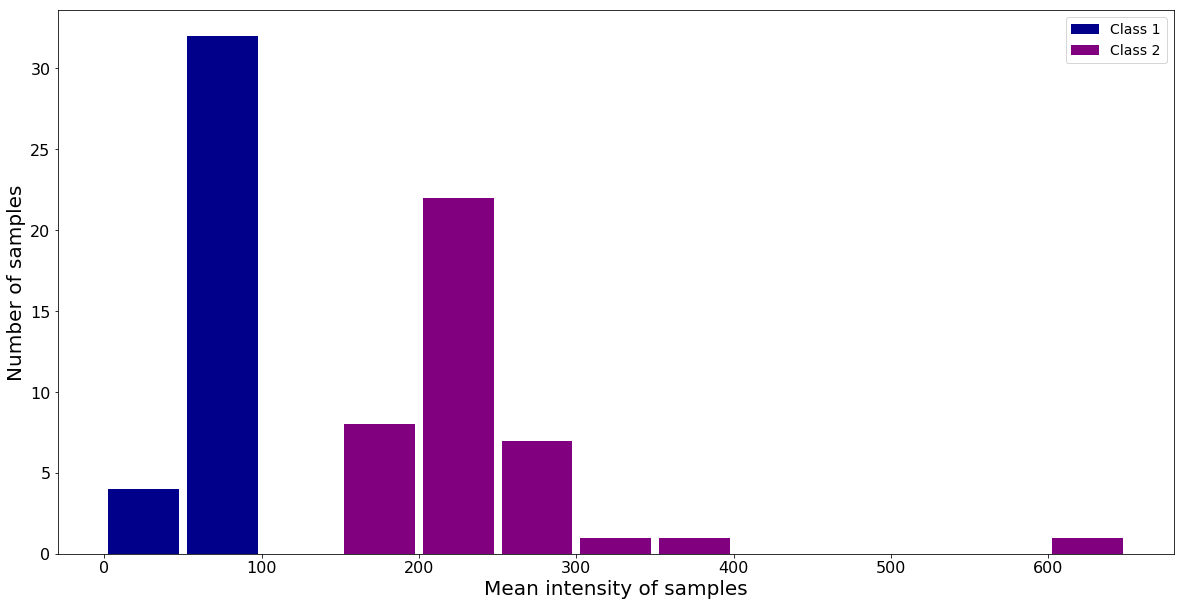
\includegraphics[width=1.0\textwidth]{imgs/intensity_distr.png}
\caption{Intensity distribution in the data set. Blue shows the Epi samples and purple shows Jopp data.}
\par
\end{figure}

In contrast to the regular use of the standard score, every image was normalized on its own mean and standard deviation instead of calculating it on the entire training data. The Jopp images featured roughly five times higher intensities than the Epi data because they were recorded on different MRI machines. Figure 9 shows two spikes in mean intensities that had to be dealt with. By normalizing each 3D image on its own values, these two distributions were unified. Furthermore, this procedure will normalize future samples on the same scale the network expects no matter what the bit depth of an image is.

This approach also has a downside. The network can no longer use the mean intensity and the standard deviation as a feature to learn from because every image will be identical according to these measures. However, these two features showed no correlation to the accuracy of a prediction, which is why it was decided to use this approach.

\subsubsection{N4 Bias Field Correction}

A bias field is a low-frequency non-uniform intensity that is an unwanted byproduct Magnetic Resonance imaging. Several methods have been developed in the past of which N4ITK is the de facto standard in the field \cite{Tustison2010}. This algorithm approximates the nonuniform field and balances intensities using B-Splines. 

\begin{figure}[H]
\minipage{0.32\textwidth}
  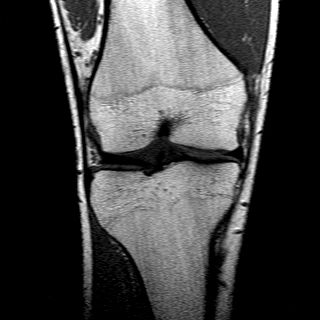
\includegraphics[width=\linewidth]{imgs/orig.jpg}
\endminipage\hfill
\minipage{0.32\textwidth}
  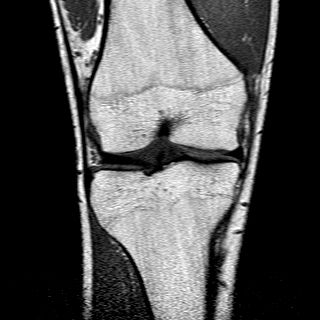
\includegraphics[width=\linewidth]{imgs/corr.jpg}
\endminipage\hfill
\minipage{0.32\textwidth}%
  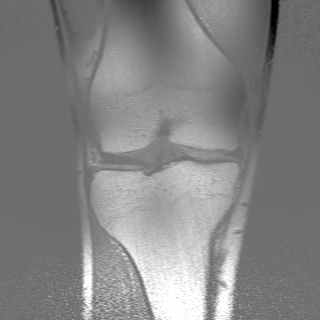
\includegraphics[width=\linewidth]{imgs/diff2.jpg}
\endminipage
\caption{Raw image (left), corrected image (middle) and visualization of intensity differences between the two (right)}
\end{figure}

As the name suggests, it is included in the Insight Toolkit (ITK) for which SimpleITK delivered an available Python binding. Using the N4 Bias Field Correction with its default settings on a single 24x224x224 image took between 60 and 120 seconds.

\subsubsection{Augmentation}

Image augmentation is a popular approach to virtually increase the size of the dataset. The general idea is that a neural network will overfit more when learning one sample n times, in comparison to learning n alternations of this sample just once. It helps to generalize on new images instead of memorizing patterns in the training data.

Lossless augmentation techniques are those that don't change the values and relative localities in a sample. In 2D these include vertical and horizontal flips, as well diagonal flips if width and height are equal. Note that any multiples of 90-degree rotations can also be created using a combination of these flips. Although the samples are changed as a whole, they do not vary concerning their contained values. 

The term "lossless" only refers to the technical change and not necessarily to the semantic change. Flipping a slice of this dataset vertically, switches the absolute positions of Femur and Tibia. This might make it harder for the network to distinguish between the two.

Lossy augmentation methods include a variety of image transformations. Common choices include:

\begin{itemize}
\item Horizontal shifts
\item Vertical shifts
\item Rotations
\item Shear mapping
\item Brightness adjustments
\item Contrast adjustments
\item Gamma adjustments
\end{itemize}

For this study horizontal flips were implemented to give the impression that images from both knees were available. In addition to this, these images were shifted 24 pixels on the horizontal axis to add another type of augmentation. 

Interestingly, these methods did not improve the accuracy of the model. The horizontal flips even hurt the performance and were therefore removed. The horizontal shifts were kept in the training set, so the network would perform better on unseen data that was not perfectly aligned.

\subsubsection{2D and 3D data}

Although convolutional neural networks are most commonly connected with 2D data such as photos or drawings, they can be applied in any dimensional space. In Natural Language Processing (NLP) 1D convolutions are often used on sentences and in finance they can be applied to time series forecasting. In the medical field where a variety of volumetric data exists, 3D convolutions have become a popular choice for building deep learning solutions.

In the context of neural networks, one has to differentiate between volumetric data with one channel and 2D data that consists of multiple color channels. Both are an example of 3D data, but the volumetric images feature three spatial dimensions, whereas photos feature only two. Convolutions commonly traverse the spatial dimensions, which means photos with multiple channels are usually not subject to 3D convolutions. Instead, various input channels are fed into a 2D CNN.

Although the data set consisted of volumetric MRI data, the z-axis showed 20 times fewer voxels than the other two dimensions. Not knowing the influence of this situation both 3D and 2D architectures were investigated for this project. The 3D model didn't use any MaxPooling on the already small z-axis. A kernel size of 3x3x3 was used similarly to the 3D version of U-Net. The 2D data was created by using each slice as a single input image.

As described in 3.3.1 the 3D convolutional network used 24x224x224 voxel images from both the Epi and Jopp data. In contrast, the 2D network used all of the available slices from each source as separate images.

While in theory, the spatial information of the z-axis gave the 3D network more contextual information of every slice, the 2D model performed better at the end. The latter was also less computationally expensive and allowed working with data where only single slices were available per sample.

\subsubsection{Separate Bone Maps}

The initial segmentation maps came with three separate channels for the Femur, Tibia, and Fibula. With this information, it was possible to train a network that would segment the three bones while still differentiating between them.

\begin{figure}[H]
\minipage{0.24\textwidth}
  
\includegraphics[width=\linewidth]{imgs/x1.png}
\endminipage\hfill
\minipage{0.24\textwidth}
  
\includegraphics[width=\linewidth]{imgs/x2.png}
\endminipage\hfill
\minipage{0.24\textwidth}%
  
\includegraphics[width=\linewidth]{imgs/x3.png}
\endminipage\hfill
\minipage{0.24\textwidth}%
  
\includegraphics[width=\linewidth]{imgs/x4.png}
\endminipage
\vspace{0.15cm}
\minipage{0.24\textwidth}
  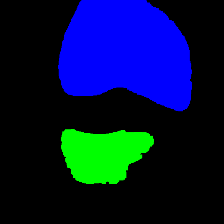
\includegraphics[width=\linewidth]{imgs/y1.png}
\endminipage\hfill
\minipage{0.24\textwidth}
  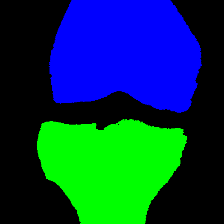
\includegraphics[width=\linewidth]{imgs/y2.png}
\endminipage\hfill
\minipage{0.24\textwidth}%
  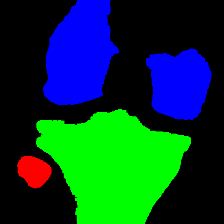
\includegraphics[width=\linewidth]{imgs/y3.png}
\endminipage\hfill
\minipage{0.24\textwidth}%
  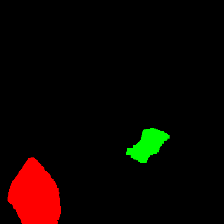
\includegraphics[width=\linewidth]{imgs/y4.png}
\endminipage
\caption{Four sample slices with their ground truth segmentations showing the three separate bones}
\end{figure}

However, this led to problems with the Fibula, which was not recognized by any of the applied architectures. The channel was always predicted empty. It's appearance in the images accounted for 3.4\% of the segmented area, whereas the Tibia made up 41\% and the Femur accounted for the remaining 55.6\%. This led the network to learn that an empty prediction of this channel is valid in 96.6\% of the cases, which is very accurate on its own. Instead of spending capacity on improving a channel that only makes up a tiny fraction of the result, the network improved the performance of Femur and Tibia.

The only successful method was training a separate model for each of the three bones. The network started to predict empty segmentation maps in the beginning because the actual masks only made up a fraction of the frame. The only way to improve from here was to find the Fibula in the non-empty slices and segment its region. This was different from the tests before, where the unsatisfactory performance of the Fibula was balanced by making more accurate segmentations of the other two bones.

For another experiment, the three channels were merged to create a network that would segment any bone in the image. Not only did this solve the problem with the Fibula as well, but the predictions of Femur and Tibia were also more accurate. The network didn't need to learn any more that the global position in the image accounts for whether or not an object should be segmented. Instead, it could segment any bone in any position in the frame. It was decided to continue with this approach for further tests, but the same architecture can be used on single bone channels as well.

\subsection{Architecture}

The majority of classification CNNs use a recurrent combination of convolutional and pooling layers \cite{Krizhevsky}\cite{He2015b}\cite{Iandola2016a}\cite{Ronneberger2015a}. By combining the local learning patterns of convolutions with the spatial reductions of pooling, the input is compressed to a dense representation of its most important features.

As mentioned in 3.2.5 a segmentation can be seen as a classification for every pixel. As such, early CNN segmentation models used small patches of the input image only to predict a single pixel through a classification pipeline. Afterward, a full segmentation map was assembled using each of these pixels. This process was very slow, and it also prevented the network to have a field of view larger than the inserted patch.

An improvement for segmentations came through architectures referred to as encoder-decoder models. The encoding process describes the same spatial compression used in classification networks. Afterward, in the decoding step, the spatial resolution is brought back to its original shape and further processed by additional convolutions. This yields huge speed improvements, while also increasing the accuracy of the prediction. Encoder-decoder networks are the de facto standard in the current field of image segmentation \cite{Chen2017}\cite{Zhao2016}\cite{Lin2016}\cite{Chen2016}\cite{Nekrasov2016}\cite{Milletari2016}\cite{Cicek2016}\cite{Ronneberger2015a}\cite{Badrinarayanan2015}, and they were the initial starting point for building architecture.

\begin{figure}[H]
\centering
\par
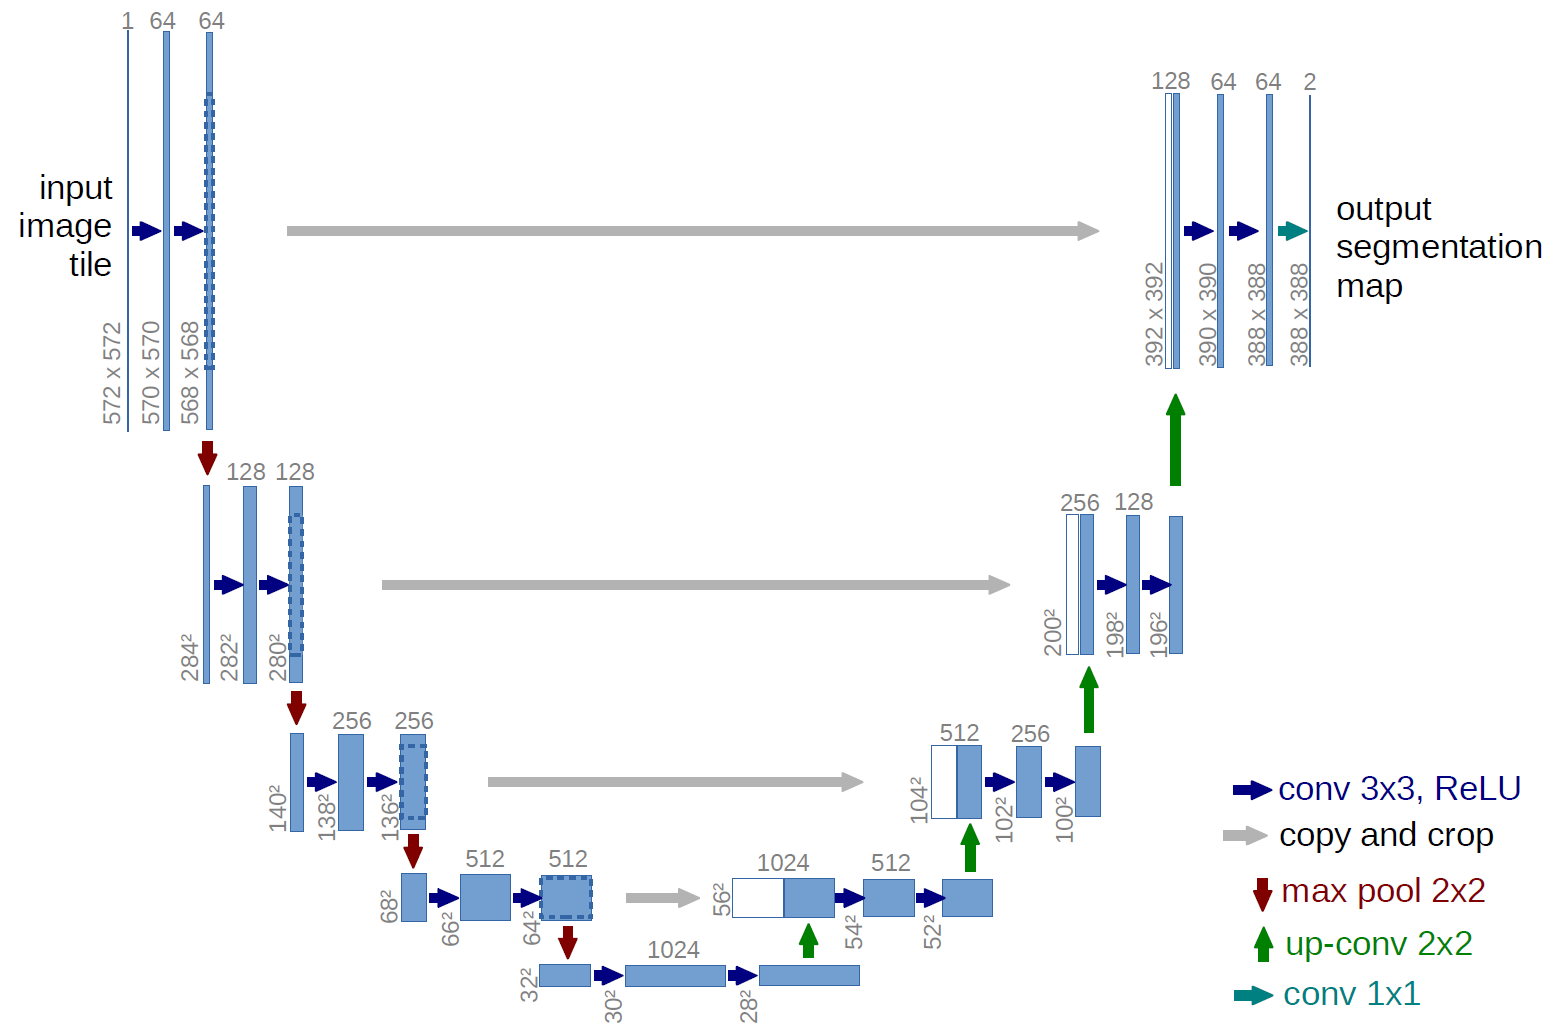
\includegraphics[width=1.0\textwidth]{imgs/unet.png}
\caption{Visualization of the U-Net architecture}
\par
\end{figure}

Figure 12 shows a particular implementation of an encoder-decoder model known as U-Net \cite{Ronneberger2015a}. It has been successfully used on a variety of projects in and outside the medical field. The contracting side on the left shows a similar architecture to classification CNNs, after which the process is mirrored on the expanding side.

The following subchapters will discuss key elements that go into the design process of such an architecture. It was also analyzed how technologies that were introduced after the U-Net paper could improve the performance on this data set.

\subsubsection{Channels, Growth Rate and Depth}

The number of parameters in a neural network has a high correlation with its learning capacity. By adding more nodes that can be adjusted during training, the model can approximate a more complex function that transforms the input into the output. The downside is that a larger parameter count will also increase the possibility of overfitting the data. A convention in the field of CNNs is to gradually increase the number of channels, while the spatial resolution is reduced due to the use of MaxPooling \cite{Krizhevsky}\cite{He2015b}\cite{Iandola2016a}\cite{Ronneberger2015a}. U-Net also shows this behavior on the left side of its architecture.

A test was set up that compared the original U-Net against five smaller variants. They varied in the total number of parameters and how the number of channels changed from one layer to the next.

\begin{table}[H]
    \centering
    \begin{tabular}{| l || r | r | r | r | r | r | r | r | r || r |}
    \hline
    Name    & C1   & C2   & C3   & C4   & C5   & C6   & C7   & C8   & C9  & Param. \\ 
    \hline
    \hline
    Model A &   32 &   32 &   32 &   32 &   32 &   32 &   32 &   32 &  32 & 211k      \\
    \hline
    Model B &   16 &   24 &   36 &   54 &   81 &   54 &   36 &   24 &  16 & 340k      \\
    \hline
    Model C &   48 &   48 &   48 &   48 &   48 &   48 &   48 &   48 &  48 & 474k      \\
    \hline
    Model D &    8 &   16 &   32 &   64 &  128 &   64 &   32 &   16 &   8 & 485k      \\
    \hline
    Model E &   32 &   48 &   72 &  108 &  159 &  108 &   72 &   48 &  32 & 1,358k      \\
    \hline
    U-Net   &   64 &  128 &  256 &  512 & 1024 &  512 &  256 &  128 &  64 & 31,000k      \\
    \hline
    \end{tabular}
    \caption{Convolution blocks 1 to 9 of the candidates with their respective output channels and total number of parameters}
\end{table}

Training U-Net was very slow in two regards. Each training step lasted six times longer compared to the smallest model, while it also took 25 times more training steps to reach the same results. Since it was also overfitting to a significant amount, it was not trained until the end. The second largest model E also overfitted on the training data and never achieved comparable results to the other four models.

D started with eight channels which were then increased by a factor of 2, whereas B started out larger but only increased the channels by a rate of 1.5. Although being the smaller model, B showed a higher accuracy in the end. It was concluded that the initial number of output channels has a larger effect on the result than the growth rate.

This theory was supported by the results from A and C, both of which kept their initial number of channels throughout the network. These two showed the highest scores in comparison to the other models while maintaining their relatively small size. Since their results were identical, model A was kept because of its faster training speed. It was interesting to see that the smallest model performed best across the candidates.

The original U-Net featured a depth of 5 convolutional blocks until reaching the bottom of the "U"-shape. It was also investigated that a depth of 6 would not improve performance, while a depth of 4 decreased the accuracy. Therefore, Model A was left unchanged.

\subsubsection{Skip Connections}

U-Net uses skip connections to copy values from the left side to the corresponding layer on the right side. This improves performance because otherwise spatial information would get lost while contracting the input. An experiment showed that removing these paths indeed hurt the performance badly.

ResNet \cite{He2015b} is another popular classification architecture that was the first to use residual connections. These are another type of skip connection that bridge the beginning and end of a convolutional block. According to the original paper, they are also one of the main reasons CNNs can be expanded to depths of thousands of layers. Since their use in the industry has found great success in many models, they were also applied in this network. However, they did not have an impact on the performance or the training speed, which is why they were not used in the end.

\subsubsection{Dropout}

Dropout is a popular regularization technique that randomly zeros out a fraction of the nodes during training \cite{Srivastava2014}. It is understood that this helps the model to generalize better and reduce overfitting on a given data set. Well known image classification architectures like VGG16 \cite{Simonyan2014a}, SqueezeNet \cite{Iandola2016a} or AlexNet \cite{Krizhevsky} use Dropout near the end of the network. Similarly, U-Net uses Dropout at the end of the contracting path to prevent overfitting.

Since a single unit of dropout with a rate of 0.5 is common in other architectures, this was also chosen as a first option. Other tests included adding multiple dropout units between the convolutions on the contracting side, which led to slower training and lower scores. Adding dropout on the expanding side is rather unusual and also didn't perform well in the tests. In the end, the first candidate was chosen for future training.

\subsubsection{Activation Functions}

Activation functions sit between layers in a network to introduce a non-linearity. Otherwise, the dense and convolutional operations could be regenerated to a simple linear transformation and remove the benefits of building a deep model.

\[
relu(x) =
\begin{cases} 
0 & \text{if } x < 0  \\
x & \text{if } x \geq 0
\end{cases}
\]

The rectified linear unit or ReLU \cite{Nair} is the default recommendation for an activation function in modern neural networks. It's defined as the maximum of 0 and the input value and can be described as a nonlinear function made up of two linear pieces. Because of this, it preserves many of the properties that make models easy to optimize and generalize well on new data \cite{Goodfellow2016}.

\[
elu(x) =
\begin{cases} 
e^x - 1 & \text{if } x < 0  \\
x & \text{if } x \geq 0
\end{cases}
\]

Since the introduction of ReLU other variants have built on its success like PReLU \cite{He2015a}, LReLU and ELU \cite{Clevert2015}. The latter titled exponential linear unit shows the same linear behavior for positive values but adds an exponential function to negative inputs instead of erasing its value.  This has shown further improvements by keeping the mean of values centered at 0 while only being slightly more computationally expensive.

\begin{figure}[H]
\centering
\par
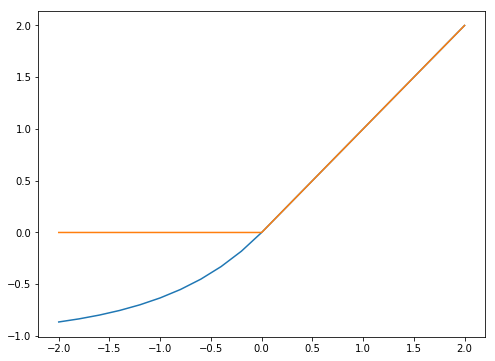
\includegraphics[width=0.5\textwidth]{imgs/elu_relu1.png}
\caption{Visualization of ReLU in orange and ELU in blue}
\par
\end{figure}

ELU showed superior results in comparison to ReLU and was chosen for all future tests.

\subsection{Training}

The training is where the actual learning takes place, and its process is inspired by how humans improve their performance on tasks. When opposed to a difficult question the first step would be a mere guess of what the answer might be. In a second phase, this information is compared to the right answer and processed by the brain accordingly.

Similarly, the training of a neural network consists of two parts. In the first step, the input is fed forward through the network, and an answer prediction is made. In the very beginning, this is just a random guess because ANNs are initialized with random values. 

\begin{figure}[H]
\centering
\par

\includegraphics[width=1.0\textwidth]{imgs/forward_backward_prop.png}
\caption{The iterative process of forward and backward propagation}
\par
\end{figure}

The prediction is then compared to the right answer, and the error is calculated. This metric can be fed back through the network to optimize the parameters in the model. These two steps are called forward and backward propagation.

\subsubsection{Metrics and Loss Functions}

Metrics are used in deep learning to measure the performance of a model. For example, the accuracy is often chosen to describe how well a neural network is doing on a classification task. An accuracy of 0.9 indicates that 9 out of 10 samples are classified correctly.

\begin{equation}
Accuracy = \frac{TP+TN}{TP+TN+FP+FN}
\end{equation}

In the formula above T and F indicate whether a prediction was true or false. P and N stand for a positive or negative outcome.

The result of a loss function is a metric that will be minimized during the backward propagation process. It needs to be a differentiable function, which is why the accuracy cannot be used as a loss function. It is a binary metric that works with true or false values and not with probabilities.

In situations like these, a surrogate function is used that has a high correlation with the target metric. For classification problems, this is often the cross entropy. Because a segmentation can be seen as a classification for every output pixel, it was also chosen as a candidate for this study.

\begin{equation}
H(p, q) = -\sum p(x) \ log \ q(x)
\end{equation}

Another option was the $F_1 score$, which is a particular implementation of the F-Measure when $ \beta $ is 1. It is also known as the DICE coefficient (DSC).

\begin{equation}
F_\beta \ score= \frac{(1 + \beta^2) TP}{(1+\beta^2)TP+\beta^2FN+FP}
\end{equation}

Although the F1 score is commonly applied as a binary measure and therefore not differentiable, a "soft" version can be used that accounts for continuous probabilities. To use it as a loss function where 0 describes the best possible outcome the $F_1 loss$ was defined as $ 1 - F_1 \ score $.

\begin{equation}
F_\beta \ loss = 1 - F_\beta \ score
\end{equation}

The value of $ \beta $ can be adjusted to change the emphasize between precision and recall. Precision describes how much of the predicted area was true, whereas recall describes how much of the ground truth was recognized by the model. This can be useful for data sets with large imbalances between classes, like this study showed between Fibula, Femur, and Tibia. 

The $F_2 score$ was tried for the three channel segmentation, where the Fibula could not be recognized. Although this model showed better scores regarding the recall measure, the Fibula was still not segmented.

\begin{equation}
Precision = \frac{TP}{TP+FP}
\end{equation}

\begin{equation}
Recall = \frac{TP}{TP+FN}
\end{equation}

\begin{equation}
Error = \frac{FP+FN}{TP+TN+FP+FN}
\end{equation}

Both loss functions were used in separate runs to compare the results of the $F_1 \ score$ and the cross entropy. The $F_1$ trained model showed better results regarding the $F_1 \ score$ and the cross entropy model showed better results on the cross entropy loss. In regards to Precision, Recall, Accuracy, and Intersection-over-Union (IoU) the performance of the $F_1$ trained network showed higher scores.

\begin{equation}
IoU= \frac{TP}{TP+FP+FN}
\end{equation}

Another test run used both loss function at the same time. This was done by feeding the output of the next-to-last layer into two separate segmentation outputs. Each of these last layers was trained with the $F_1 \ loss$ and cross entropy loss respectively. All previous layers were therefore trained by the sum of both loss functions. This architecture matched the best results of the previous runs in a single model but also increased the training time by 30\%.

Evaluating these two outputs on the other metrics played in favor for the $F_1 loss$ output. Combining both maps didn't improve the scores any further. Since the cross entropy was chosen as a surrogate function and not as a performance metric, all future tests used only the $F_1 loss$. This delivered faster training than the dual output method.

\subsubsection{Optimizer}

The previous chapter provided an overview of the loss function, which measures the performance of a prediction during the training process. This chapter discusses how the result can be used to execute the actual optimization step.

The derivative of a single variable function defines the slope of this function at any given point. Knowing this, one can tell in which direction the original function declines. Adjusting the independent variable along the descent of a loss function will minimize the error in respect to its dependent variable.

The gradient is the derivative for functions of multi-dimensional inputs, such as the loss functions used in deep learning. A process that minimizes its result is called gradient descent. While it is possible to determine its minimum analytically, it is intractable for artificial neural networks due to the high number of parameters \cite{Chollet2017}.

Instead, the stochastic gradient descent (SGD) is used which will take a random batch of the training data and iteratively adjust the parameters in small steps. SGD is the basis for all common ANNs, but over the years different variants were introduced to the field.

The Adam optimizer \cite{Kingma2014} is such a variant, which enhances SGD amongst other things by using what's called an "adaptive momentum estimation." This is also where its name derives from. It adaptively adjusts the learning rate which defines how much the parameters will be changed in one training step. By incorporating the previous and current shape of the slope, Adam can tremendously speed up the training.

\subsubsection{Batch Size}

The number of random samples per training step is referred to as the batch size. In the past, it was believed that larger batches led to something called the generalization gap \cite{Keskar2016}, where the accuracy of a model would drop if it was trained on unusually large batches. Recent work \cite{Hoffer2017} suggests other reasons for this decrease in accuracy. While common batch sizes range from 32 to 256, Goyal et al. showed accurate results using 8192 images per batch when training a model on ImageNet \cite{Goyal2017}.

Using batches smaller than 32 samples can introduce a different kind of problem. Having too few data points that don't represent the mean of the data well, may lead to slow and unstable training.

Based on hardware limitations the largest possible batch sizes ranged from 24 to 48 samples depending on the current architecture. Whatever could be fit into memory was used for these experiments. Exceptions occurred when working with 3D convolutions in which case the batch size had to be limited to just 4 samples.

\subsubsection{Learning Rate Policy}

One full iteration over the training samples is referred to as an epoch, and the learning rate policy describes how the learning rate is changed from one epoch to another. With the introduction of adaptive optimizers like Adam or RMSProp, there has been a lower emphasize on this topic. Learning rates that were set too high or too low will be adjusted by the optimizer after a few iterations. Even though this reduces the number of possible defects, a lot of training time can be saved with the right policy.

Ten epochs were run at different learning rates to compare initial results and to examine the point at which the model wouldn't converge at all. 0.002 was the highest rate at which the model started training, but 0.001 resulted in the best score.

\begin{figure}[H]
\[
lr(x) = \frac{1}{1 + decay * x}
\]
\caption{Learning rate at epoch x based on the decay value}
\end{figure}

After the model had stopped to improve at epoch 65, the learning rate was changed to 0.0001. This gave a small boost of accuracy. To have a smooth transition between learning rates, the decay was set to 0.001. This meant that the initial learning rate of 0.001 would reach 0.0001 after 68 epochs and then continue to decrease even further.

\subsubsection{Early Stopping}

Neural networks will continuously minimize the loss on the training set. This result needs to be validated on data the network hasn't seen before. At a certain point during training, the performance on the validation set will start to decrease because the model is overfitting on the training data. The number of iterations to reach this point is dependent on many hyperparameters, as well as the random values the network has been initialized with. As such it's difficult to calculate how many epochs the training will need to reach its peak.

Early stopping is a simple technique that will end the training process as soon as the model stops improving on the validation data. To do this, a patience value is defined how long the network should continue training after the score has stopped increasing. This is important because not every epoch will lead to a new best score on the validation data.

For test runs in this study, a patience of 9 was selected, which meant the training would stop after 10 epochs without improvement. Depending on the architecture and other hyperparameters this point was reached after 50 to 90 epochs. For the last training with the final set of hyperparameters, the patience was increased to 19, which didn't improve the accuracy.  This was also a verification that the initial value of 9 was a good fit for this problem.

\subsection{Summary}

In summary, the architecture features 4 "Down Blocks" on the contracting side that are mirrored through 4 "Up Blocks" on the expanding side. Each level is connected to the other side to share information at the current spatial resolution.

\begin{figure}[H]
\centering
\par

\includegraphics[width=0.55\textwidth]{imgs/model.png}
\caption{The proposed architecture for the segmentation}
\par
\end{figure}

A Down Block consists of 2 convolutional layers each followed by an ELU activation function, after which A MaxPooling layer halves the width and height of the image. The Up Block looks similar but features a transposed convolutional layer in the beginning to upsample the resolution and no MaxPooling in the end. The Middle Block features a Dropout layer with a value of 0.5, which is surrounded by convolutional layers as well. All convolutional layers have 32 channels. The output layer includes another convolution that reduces the channels to 1, which represents the segmentation map.

Other options that were tried but didn't improve performance included using convolutional blocks with a stride of 2 instead of MaxPooling to downsample the images. Batch normalization was also applied but resulted in a high amount of overfitting the network never recovered from. The fact that it did not improve the performance came as a surprise because it usually improves any model. A possible reason for this could be the small batch size in combination with a high variance of intensities in the data. If the mean of each batch varies significantly from the mean of the entire training data, it may hurt the performance of batch normalization.

\newpage

\section{Results}

The results in this chapter are based data the network has not been trained with. It was also made sure that there was no overlap in images of people that were recorded multiple times. Five images were chosen randomly from each of the two sources in the very beginning. Since the Epi data featured 41 slices and the Jopp data featured 24 slices, 325 2D samples were available for evaluation. Each slice contained 50,176 pixel values, making a total of 16.3 million predictions that were analyzed.

The network architecture was developed using a single segmentation channel that merged Femur, Tibia and Fibula maps. However, tests were also run to validate the performance for each bone on its own and also combine the three separate predictions into a multi channel segmentation. The same architecture and training procedure was used for this task.

\subsection{Numeric Evaluation}

The proposed model achieves a DSC score of 98.0\% and an IoU of 96.0\%. Precision and Recall are perfectly balanced at 98.0\% as well, suggesting that predictions are neither too optimistic or pessimistic. The error shows a small value of 1.2\%.

\begin{table}[H]
    \centering
    \begin{tabular}{| l | c | c | c | c | c |}
    \hline
           & DSC & IoU & Precision & Recall & Error \\ 
    \hline
    Merged   & \makecell{0.980} 
             & \makecell{0.960} 
             & \makecell{0.980} 
             & \makecell{0.980} 
             & \makecell{0.012} \\
    \hline
    Femur    & \makecell{0.981} 
             & \makecell{0.963} 
             & \makecell{0.979} 
             & \makecell{0.984} 
             & \makecell{0.006} \\
    \hline
    Tibia    & \makecell{0.977} 
             & \makecell{0.955} 
             & \makecell{0.976} 
             & \makecell{0.977} 
             & \makecell{0.006} \\
    \hline
    Fibula   & \makecell{0.953} 
             & \makecell{0.911} 
             & \makecell{0.954} 
             & \makecell{0.952} 
             & \makecell{0.001} \\
    \hline
    Combined & \makecell{0.979} 
             & \makecell{0.958} 
             & \makecell{0.977} 
             & \makecell{0.981} 
             & \makecell{0.004} \\
    \hline
    \end{tabular}
    \caption{Numeric evaluation of the test set using popular metrics}
\end{table}

Results on Femur and Tibia alone are comparable to the merged approach, whereas the Fibula segmentation reaches a DSC of 95.3\% and IoU of 91.1\%. This could be due to the fact that the Fibula is only visible in a minority of slices, making it a somewhat unbalanced task. Combining the three separate segmentations to a single model gives comparable results as well. The error is even reduced by a factor of 3, which is expected because the segmentation channels are increased by 3.

A study from 2011 ran a similar segmentation on the knee \cite{Martel-Pelletier2011}, achieving a DSC of 94\% for the femur and 92\% for the tibia using the ray casting technique. Another study from 2015 \cite{Dam} used an atlas based segmentation and achieved a DSC of 97.5\% for the tibia.

\subsection{Visual Evaluation}

The visual evaluation will focus on the results of the combined network since its performance is on par with the one channel model while offering more information about the associated bones.

The network shows excellent performance on slices that are located near the middle of the 3D MRIs with DSC scores of over 99\%.

\begin{figure}[H]
\minipage{0.24\textwidth}
  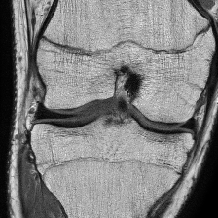
\includegraphics[width=\linewidth]{imgs/a1.png}
\endminipage\hfill
\minipage{0.24\textwidth}
  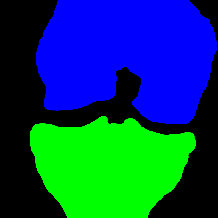
\includegraphics[width=\linewidth]{imgs/b1.png}
\endminipage\hfill
\minipage{0.24\textwidth}%
  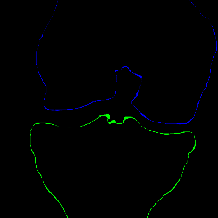
\includegraphics[width=\linewidth]{imgs/c1.png}
\endminipage\hfill
\minipage{0.24\textwidth}%
  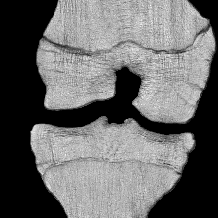
\includegraphics[width=\linewidth]{imgs/d1.png}
\endminipage
\vspace{0.15cm}
\minipage{0.24\textwidth}
  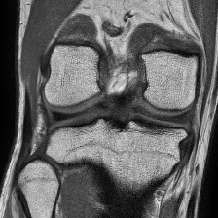
\includegraphics[width=\linewidth]{imgs/a2.png}
\endminipage\hfill
\minipage{0.24\textwidth}
  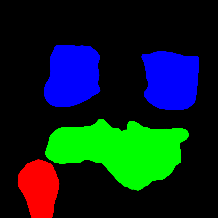
\includegraphics[width=\linewidth]{imgs/b2.png}
\endminipage\hfill
\minipage{0.24\textwidth}%
  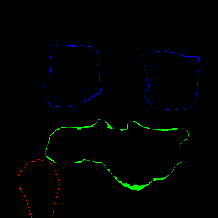
\includegraphics[width=\linewidth]{imgs/c2.png}
\endminipage\hfill
\minipage{0.24\textwidth}%
  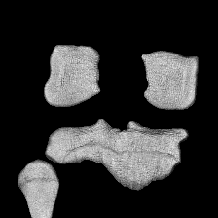
\includegraphics[width=\linewidth]{imgs/d2.png}
\endminipage
\vspace{0.15cm}
\minipage{0.24\textwidth}
  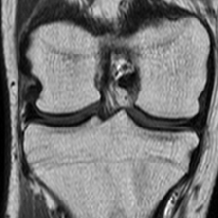
\includegraphics[width=\linewidth]{imgs/a3.png}
\endminipage\hfill
\minipage{0.24\textwidth}
  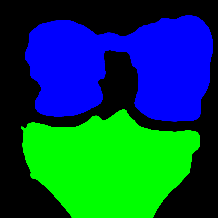
\includegraphics[width=\linewidth]{imgs/b3.png}
\endminipage\hfill
\minipage{0.24\textwidth}%
  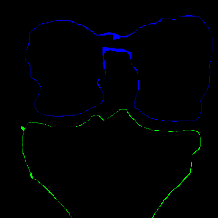
\includegraphics[width=\linewidth]{imgs/c3.png}
\endminipage\hfill
\minipage{0.24\textwidth}%
  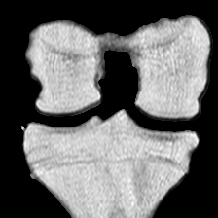
\includegraphics[width=\linewidth]{imgs/d3.png}
\endminipage
\vspace{0.15cm}
\minipage{0.24\textwidth}
  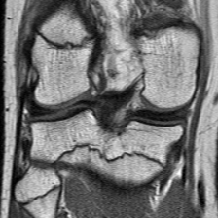
\includegraphics[width=\linewidth]{imgs/a4.png}
\endminipage\hfill
\minipage{0.24\textwidth}
  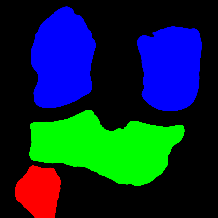
\includegraphics[width=\linewidth]{imgs/b4.png}
\endminipage\hfill
\minipage{0.24\textwidth}%
  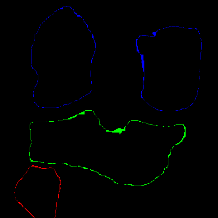
\includegraphics[width=\linewidth]{imgs/c4.png}
\endminipage\hfill
\minipage{0.24\textwidth}%
  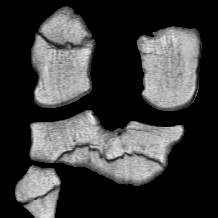
\includegraphics[width=\linewidth]{imgs/d4.png}
\endminipage
\caption{Random slices extracted from the middle of the 3D images. Each row shows input, predicted output, difference to ground truth and applied mask to input}
\end{figure}

Perfect DSC scores of 100\% are achieved through empty segmentations that the network correctly predicted as such.

\begin{figure}[H]
\minipage{0.24\textwidth}
  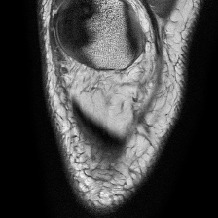
\includegraphics[width=\linewidth]{imgs/a5.png}
\endminipage\hfill
\minipage{0.24\textwidth}
  
\includegraphics[width=\linewidth]{imgs/b5.png}
\endminipage\hfill
\minipage{0.24\textwidth}%
  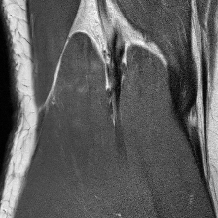
\includegraphics[width=\linewidth]{imgs/a6.png}
\endminipage\hfill
\minipage{0.24\textwidth}%
  
\includegraphics[width=\linewidth]{imgs/b6.png}
\endminipage
\caption{One upper and lower slice example of a correctly predicted empty segmentation.}
\end{figure}

The most imprecise predictions also appeared in upper and lower slices where the bones started to become visible. If either the prediction or the ground truth was empty while the other was not, then the result is a DSC score of 0\%.

\begin{figure}[H]
\minipage{0.32\textwidth}
  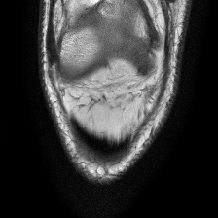
\includegraphics[width=\linewidth]{imgs/a8.png}
\endminipage\hfill
\minipage{0.32\textwidth}
  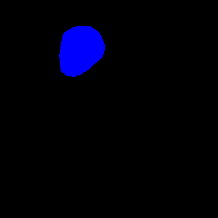
\includegraphics[width=\linewidth]{imgs/b8.png}
\endminipage\hfill
\minipage{0.32\textwidth}%
  
\includegraphics[width=\linewidth]{imgs/c8.png}
\endminipage
\vspace{0.2cm}
\minipage{0.32\textwidth}
  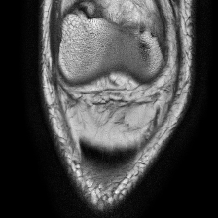
\includegraphics[width=\linewidth]{imgs/a7.png}
\endminipage\hfill
\minipage{0.32\textwidth}
  \includegraphics[width=\linewidth]{imgs/b7.png}
\endminipage\hfill
\minipage{0.32\textwidth}%
  \includegraphics[width=\linewidth]{imgs/c7.png}
\endminipage
\caption{Two examples of falsely predicted estimates whether or not the bone is already visible. Each row shows input, ground truth and prediction}
\end{figure}

In these examples, the ground truth defines the Femur to be visible in the upper image but not in the one below it. The prediction disagrees with it in both cases. These are two examples that could be seen as noise in the ground truth data or to be debatable at least.

\subsection{Model Exploration}

Neural networks are often considered black boxes because it is difficult to get an intuitive understanding how decisions are calculated. This is a crucial problem especially in the medical field, where a prediction may approximate certain health conditions about a patient.

Two factors help in this study to pull away from this problem. Firstly, a segmentation is an image to image pipeline making it less abstract what kind of transformations are happening. Visualizing input and output gives an intuitive understanding how one may have emerged out of the other.

Secondly, convolutional neural networks take away most of this black box reasoning \cite{Chollet2017} because every layer in the network can be visualized. The following images give an insight what a sample looks like after different convolutional blocks.

\begin{figure}[H]
\minipage{0.24\textwidth}
  \includegraphics[width=\linewidth]{imgs/a_input.png}
\endminipage\hfill
\minipage{0.24\textwidth}
  \includegraphics[width=\linewidth]{imgs/down1.png}
\endminipage\hfill
\minipage{0.24\textwidth}%
  \includegraphics[width=\linewidth]{imgs/down2.png}
\endminipage\hfill
\minipage{0.24\textwidth}%
  \includegraphics[width=\linewidth]{imgs/down3.png}
\endminipage
\vspace{0.15cm}
\minipage{0.24\textwidth}
  \includegraphics[width=\linewidth]{imgs/down4.png}
\endminipage\hfill
\minipage{0.24\textwidth}
  \includegraphics[width=\linewidth]{imgs/middle1.png}
\endminipage\hfill
\minipage{0.24\textwidth}%
  \includegraphics[width=\linewidth]{imgs/middle2.png}
\endminipage\hfill
\minipage{0.24\textwidth}%
  \includegraphics[width=\linewidth]{imgs/up1.png}
\endminipage
\vspace{0.15cm}
\minipage{0.24\textwidth}
  \includegraphics[width=\linewidth]{imgs/up2.png}
\endminipage\hfill
\minipage{0.24\textwidth}
  \includegraphics[width=\linewidth]{imgs/up3.png}
\endminipage\hfill
\minipage{0.24\textwidth}%
  \includegraphics[width=\linewidth]{imgs/up4.png}
\endminipage\hfill
\minipage{0.24\textwidth}%
  \includegraphics[width=\linewidth]{imgs/z_output.png}
\endminipage
\caption{Intermediate feature maps of the convolutional blocks in the proposed architecture. Each is the sum of the 32 individual output channels}
\end{figure}

Each image shows the sum of all intermediate channels at a particular layer. The first image is the raw input, whereas the last image is the final segmentation map. One can clearly see the reduction of resolution towards the middle, which is then brought back up. The first convolutional block inverses the input and removes most of the bone structure except for the growth plates. The second to last output looks similar to the input, but the skin on the sides is almost entirely removed, and the dark growth plates have been filled. Looking closer at this image one can also notice a crisp black line that separates the bone from the rest. A simple threshold at this point would segment the bone fairly accurate.

Even at this level, it is difficult to judge what exactly the network is detecting. For another visualization, the intermediate channels are not added like before but analyzed separately.

\begin{figure}[H]
\minipage{0.24\textwidth}
  \includegraphics[width=\linewidth]{imgs/channel1.png}
\endminipage\hfill
\minipage{0.24\textwidth}
  \includegraphics[width=\linewidth]{imgs/channel3.png}
\endminipage\hfill
\minipage{0.24\textwidth}%
  \includegraphics[width=\linewidth]{imgs/channel2.png}
\endminipage\hfill
\minipage{0.24\textwidth}%
  \includegraphics[width=\linewidth]{imgs/channel4.png}
\endminipage
\caption{Four examples of output channels at different positions in the network}
\end{figure}

These are a few notable examples inside the model. The first filter detects high frequencies in the bone and skin tissue. Filter 2 finds vertical edges while filter 3 shows horizontal ones. Finally, filter 4 appears to be a growth plate detector. It does not just detect horizontal edges, but only those inside the bone. This seems reasonable because the network needs to learn that the dark growth plates shouldn't be interpreted as edges.


\subsection{Transfer Application}

Neural networks are known to be unreliable when used on data that exceeds the range of variation in the training set. They cannot learn what they weren't taught. On the other hand, convolutions are translation invariant, allowing them to recognize patterns anywhere in the frame \cite{Chollet2017}. Another merged model was trained that used the same architecture but added further image augmentation of horizontal and vertical flips. This way it only reached a DSC score of 97.3\% but was more flexible to structural differences in the image.

The proposed architecture can be described as "fully convolutional" because it doesn't include any dense layers. This allows the network to accept any resolution and still being able to process it. An experiment was set up that used uncropped images from the Epi data which were resized to 448x448 pixels. This made them four times larger than the images the network was trained with.

\begin{figure}[H]
\minipage{0.24\textwidth}
  \includegraphics[width=\linewidth]{imgs/transfer_size_x1.png}
\endminipage\hfill
\minipage{0.24\textwidth}
  \includegraphics[width=\linewidth]{imgs/transfer_size_x2.png}
\endminipage\hfill
\minipage{0.24\textwidth}%
  \includegraphics[width=\linewidth]{imgs/transfer_size_x3.png}
\endminipage\hfill
\minipage{0.24\textwidth}%
  \includegraphics[width=\linewidth]{imgs/transfer_size_x4.png}
\endminipage
\vspace{0.15cm}
\minipage{0.24\textwidth}
  \includegraphics[width=\linewidth]{imgs/transfer_size_y1.png}
\endminipage\hfill
\minipage{0.24\textwidth}
  \includegraphics[width=\linewidth]{imgs/transfer_size_y2.png}
\endminipage\hfill
\minipage{0.24\textwidth}%
  \includegraphics[width=\linewidth]{imgs/transfer_size_y3.png}
\endminipage\hfill
\minipage{0.24\textwidth}%
  \includegraphics[width=\linewidth]{imgs/transfer_size_y4.png}
\endminipage
\caption{Four random samples uncropped of Epi data segmentations that were resized to 448x448 pixels}
\end{figure}

The predictions look surprisingly good even following the shaft of the bone which wasn't visible in the original cropped images. Even large intensity gaps through growth plates are recognized as Femur or Tibia. The recall performance is very accurate based on a subjective visual evaluation of random samples. Problems are visible in tissue that isn't bone but was recognized as such as the 4th examples shows.

In 3.2 a third data source was mentioned that featured five sagittal recordings of knees. These were not used for the training because of their structural differences and because no ground truth segmentations were available. The following samples show what happens when the network is applied to images from a different perspective.

\begin{figure}[H]
\minipage{0.24\textwidth}
  \includegraphics[width=\linewidth]{imgs/transfer_pers_x1.png}
\endminipage\hfill
\minipage{0.24\textwidth}
  \includegraphics[width=\linewidth]{imgs/transfer_pers_x2.png}
\endminipage\hfill
\minipage{0.24\textwidth}%
  \includegraphics[width=\linewidth]{imgs/transfer_pers_x3.png}
\endminipage\hfill
\minipage{0.24\textwidth}%
  \includegraphics[width=\linewidth]{imgs/transfer_pers_x4.png}
\endminipage
\vspace{0.15cm}
\minipage{0.24\textwidth}
  \includegraphics[width=\linewidth]{imgs/transfer_pers_y1.png}
\endminipage\hfill
\minipage{0.24\textwidth}
  \includegraphics[width=\linewidth]{imgs/transfer_pers_y2.png}
\endminipage\hfill
\minipage{0.24\textwidth}%
  \includegraphics[width=\linewidth]{imgs/transfer_pers_y3.png}
\endminipage\hfill
\minipage{0.24\textwidth}%
  \includegraphics[width=\linewidth]{imgs/transfer_pers_y4.png}
\endminipage
\caption{Four random samples of sagittal Maas data segmentations using the coronal trained model}
\end{figure}

Subjectively, these results look excellent. In example 4 it even recognizes the Patella, a bone it was never trained on. This shows that with enough image augmentation the network will learn to segment any bone.

\subsection{Age Prediction}

The initial cause for the segmentation experiment was to reduce the amount of information in a knee MRI. The resulting images could then be used to make age related predictions that focussed on the bone and the growth plate. This section will briefly cover such an age prediction pipeline.

The age of the candidates ranged from 14 to 21 years with a mean at 17.5 years. Predicting this age for every person meant that it was never off more than 3.5 years. Since the data was normally distributed, a static prediction of the mean led to a mean absolute error (MAE) of 1.2 years.

Even by using many of the techniques mentioned in previous chapters, I was not able to train a stable model that could beat this baseline on the raw input data. After the segmentation maps had been applied to all 145 3D samples, many of the slices were completely empty because they didn't contain any of the three bones. It was decided to only use the middle 18 slices from each of the two sources. Out of these resulting 2610 slices, 2124 were used for the training set, but the network still wouldn't converge.

Only after using the contracting side of the proposed model with the parameters it learned on the segmentation task was I able to train a network in a stable manner. This approach did not make the model converge every time, but when it did its predictions were stable through multiple epochs.

The results on the test data showed an MAE of 0.66 years for all of the slices. Since every 3D sample now had 18 different predictions, I build another tree based model that would take a vector of 18 values and predict a single age. This got a final MAE of 0.55 years on the test data, which is more than twice as good as the baseline.

\newpage
\section{Discussion}

In this thesis


what they did (briefly)

what they found
what were the significant, memorable findings?
what do the findings mean?
what does it mean that X was rated as 4.61 and Y was rated as 3.93?
do the best of your knowledge, why do you think that is? what accounts for these results?
why are the findings significant/important/useful? how can they be used, and who can use them?

\newpage

\bibliography{references.bib}
\bibliographystyle{plain}


\end{document}